\documentclass[c]{beamer}
\setbeamerfont{footnote}{size=\tiny}
\graphicspath{{figures/}}
\setbeamertemplate{footnote}{%
  \parindent 1em\noindent%
  \raggedright
  \insertfootnotetext\par%
}
\setbeamertemplate{navigation symbols}{}
%% Этот шаблон документа разработан в 2014 году
% Данилом Фёдоровых (danil@fedorovykh.ru) 
% для использования в курсе 
% <<Документы и презентации в \LaTeX>>, записанном НИУ ВШЭ
% для Coursera.org: http://coursera.org/course/latex .
% Исходная версия шаблона --- 
% https://www.writelatex.com/coursera/latex/5.3

% В этом документе преамбула

\usepackage{siunitx}
%%% Работа с русским языком
%\usepackage{cmap}					% поиск в PDF
%\usepackage{mathtext} 				% русские буквы в формулах
%\usepackage[T2A]{fontenc}			% кодировка
%\usepackage[utf8]{inputenc}			% кодировка исходного текста
%\usepackage[english,russian]{babel}	% локализация и переносы
%\usepackage{indentfirst}
%\frenchspacing
%
%\renewcommand{\epsilon}{\ensuremath{\varepsilon}}
%\newcommand{\phibackup}{\ensuremath{\phi}}
%\renewcommand{\phi}{\ensuremath{\varphi}}
%\renewcommand{\varphi}{\ensuremath{\phibackup}}
%\renewcommand{\kappa}{\ensuremath{\varkappa}}
%\renewcommand{\le}{\ensuremath{\leqslant}}
%\renewcommand{\leq}{\ensuremath{\leqslant}}
%\renewcommand{\ge}{\ensuremath{\geqslant}}
%\renewcommand{\geq}{\ensuremath{\geqslant}}
%\renewcommand{\emptyset}{\varnothing}
%\renewcommand{\Im}{\operatorname{Im}}
%\renewcommand{\Re}{\operatorname{Re}}


%%% Дополнительная работа с математикой
\usepackage{amsmath,amsfonts,amssymb,amsthm,mathtools} % AMS
%\usepackage{icomma} % "Умная" запятая: $0,2$ --- число, $0, 2$ --- перечисление

%% Номера формул
%\mathtoolsset{showonlyrefs=true} % Показывать номера только у тех формул, на которые есть \eqref{} в тексте.
%\usepackage{leqno} % Нумереация формул слева

%% Свои команды
\DeclareMathOperator{\sgn}{\mathop{sgn}}
\DeclareMathOperator{\sign}{\mathop{sign}}
\DeclareMathOperator*{\res}{\mathop{res}}
\DeclareMathOperator*{\tr}{\mathop{tr}}
\DeclareMathOperator*{\rot}{\mathop{rot}}
\DeclareMathOperator*{\divop}{\mathop{div}}
\DeclareMathOperator*{\grad}{\mathop{grad}}

%% Перенос знаков в формулах (по Львовскому)
\newcommand*{\hm}[1]{#1\nobreak\discretionary{}
{\hbox{$\mathsurround=0pt #1$}}{}}

%%% Работа с картинками
\usepackage{graphicx}  % Для вставки рисунков
\graphicspath{{figures/}}  % папки с картинками
\setlength\fboxsep{3pt} % Отступ рамки \fbox{} от рисунка
\setlength\fboxrule{1pt} % Толщина линий рамки \fbox{}
\usepackage{wrapfig} % Обтекание рисунков текстом

%%% Работа с таблицами
\usepackage{array,tabularx,tabulary,booktabs} % Дополнительная работа с таблицами
\usepackage{longtable}  % Длинные таблицы
\usepackage{multirow} % Слияние строк в таблице

%%% Теоремы
\theoremstyle{plain} % Это стиль по умолчанию, его можно не переопределять.
\newtheorem{thm}{Теорема}
\newtheorem*{thm*}{Теорема}
\newtheorem{prop}{Предложение}
\newtheorem*{prop*}{Предложение}
 
\theoremstyle{definition} % "Определение"
%\newtheorem{corollary}{Следствие}[theorem]
\newtheorem{dfn}{Определение}
\newtheorem*{dfn*}{Определение}
\newtheorem{prob}{Задача}
\newtheorem*{prob*}{Задача}

 
\theoremstyle{remark} % "Примечание"
\newtheorem*{sol}{Решение}
\newtheorem*{rem}{Замечание}

%%% Программирование
\usepackage{etoolbox} % логические операторы

%%% Страница
%\usepackage{extsizes} % Возможность сделать 14-й шрифт
%\usepackage{geometry} % Простой способ задавать поля
%	\geometry{top=25mm}
%	\geometry{bottom=35mm}
%	\geometry{left=35mm}
%	\geometry{right=20mm}
 
\usepackage{fancyhdr} % Колонтитулы
%	\pagestyle{fancy}
 %	\renewcommand{\headrulewidth}{0pt}  % Толщина линейки, отчеркивающей верхний колонтитул
	%\lfoot{Нижний левый}
	%\rfoot{Нижний правый}
	%\rhead{Верхний правый}
	%\chead{Верхний в центре}
	%\lhead{Верхний левый}
	%\cfoot{Нижний в центре} % По умолчанию здесь номер страницы

\usepackage{setspace} % Интерлиньяж
%\onehalfspacing % Интерлиньяж 1.5
%\doublespacing % Интерлиньяж 2
%\singlespacing % Интерлиньяж 1

\usepackage{lastpage} % Узнать, сколько всего страниц в документе.

\usepackage{soul} % Модификаторы начертания

\usepackage{hyperref}
\usepackage[usenames,dvipsnames,svgnames,table,rgb]{xcolor}
\hypersetup{				% Гиперссылки
    unicode=true,           % русские буквы в раздела PDF
    pdftitle={Заголовок},   % Заголовок
    pdfauthor={Автор},      % Автор
    pdfsubject={Тема},      % Тема
    pdfcreator={Создатель}, % Создатель
    pdfproducer={Производитель}, % Производитель
    pdfkeywords={keyword1} {key2} {key3}, % Ключевые слова
%    colorlinks=true,       	% false: ссылки в рамках; true: цветные ссылки
    %linkcolor=red,          % внутренние ссылки
    %citecolor=black,        % на библиографию
    %filecolor=magenta,      % на файлы
    %urlcolor=cyan           % на URL
}

\usepackage{csquotes} % Еще инструменты для ссылок

%\usepackage[style=apa,maxcitenames=2,backend=biber,sorting=nty]{biblatex}

\usepackage{multicol} % Несколько колонок

\usepackage{tikz} % Работа с графикой
\usepackage{pgfplots}
\usepackage{pgfplotstable}
%\usepackage{coloremoji}
\usepackage{floatrow}
\usepackage{subcaption}
\graphicspath{{figures/}}

\renewcommand\thesubfigure{\asbuk{subfigure}}
%\addbibresource{master.bib}

\usepackage{import}
\usepackage{pdfpages}
\usepackage{transparent}
\usepackage{xcolor}
\usepackage{xifthen}

\newcommand{\incfig}[2][1]{%
    \def\svgwidth{#1\columnwidth}
    \import{./figures/}{#2.pdf_tex}
}
%\usepackage{titlesec}
%\titleformat{\section}{\normalfont\Large\bfseries}{}{0pt}{}
%----------------------STANDART:
%\titleformat{\chapter}[display]
%  {\normalfont\huge\bfseries}{\chaptertitlename\ \thechapter}{20pt}{\Huge}
%\titleformat{\section}{\normalfont\Large\bfseries}{\thesection}{1em}{}
%\titleformat{\subsection}
%  {\normalfont\large\bfseries}{\thesubsection}{1em}{}
%\titleformat{\subsubsection}
%  {\normalfont\normalsize\bfseries}{\thesubsubsection}{1em}{}
%\titleformat{\paragraph}[runin]
%  {\normalfont\normalsize\bfseries}{\theparagraph}{1em}{}
%\titleformat{\subparagraph}[runin]
%  {\normalfont\normalsize\bfseries}{\thesubparagraph}{1em}{}

\pdfsuppresswarningpagegroup=1
\pgfplotsset{compat=1.16}



%\setcounter{tocdepth}{1} % only parts,chapters,sections
%\titleformat{\subsection}{\normalfont\large\bfseries}{}{0em}{}
%\titleformat{\subsubsection}{\normalfont\normalsize\bfseries}{}{0em}{}

%\newcommand{\textover}[2]{\stackrel{\mathclap{\normalfont\mbox{#2}}}{#1}}

\author{Yaroslav Drachov\\
Moscow Institute of Physics and Technology}
%\author{Драчов Ярослав\\
%Факультет общей и прикладной физики МФТИ}
\newcommand{\veq}{\mathrel{\rotatebox{90}{$=$}}}
%\newcommand{\teto}[1]{\stackrel{\mathclap{\normalfont\tiny\mbox{#1}}}{\to}}
%\renewcommand{\thesubsection}{\arabic{subsection}}

%%\setcounter{secnumdepth}{0}

\definecolor{tabblue}{RGB}{30, 119, 180}
\definecolor{taborange}{RGB}{255, 127, 15}
\definecolor{tabgreen}{RGB}{45, 160, 43}
\definecolor{tabred}{RGB}{214, 38, 40}
\definecolor{tabpurple}{RGB}{148, 103, 189}
\definecolor{tabbrown}{RGB}{140, 86, 76}
\definecolor{tabpink}{RGB}{227, 119, 193}
\definecolor{tabgray}{RGB}{127, 127, 127}
\definecolor{tabolive}{RGB}{188, 189, 33}
\definecolor{tabcyan}{RGB}{22, 190, 207}
\pgfplotscreateplotcyclelist{colorbrewer-tab}{
{tabblue},
{taborange},
{tabgreen},
{tabred},
{tabpurple},
{tabbrown},
{tabpink},
{tabgray},
{tabolive},
{tabcyan},
}
\usepackage{csvsimple}
\usepackage{extarrows}
%\renewcommand{\labelenumii}{\asbuk{enumii})}
%\renewcommand{\labelenumiv}{\Asbuk{enumiv}}
%\newcommand{\prob}[1]{\subsubsection*{#1}}
\sisetup{output-decimal-marker = {,},separate-uncertainty = true,exponent-product = \cdot}

\usepackage{braket}
\usepackage{enumerate}
\usepackage{chngcntr}
%\counterwithin*{equation}{problem}
%\usepackage{bbold}

\newtheoremstyle{hiProb}% ⟨name ⟩ 
{3pt}% ⟨Space above ⟩1 
{3pt}% ⟨Space below ⟩1
{}% ⟨Body font ⟩
{}% ⟨Indent amount ⟩2
{\bfseries}% ⟨Theorem head font⟩
{.}% ⟨Punctuation after theorem head ⟩
{.5em}% ⟨Space after theorem head ⟩3
%{\thmname{#1} \thmnote{#3}}% ⟨Theorem head spec (can be left empty, meaning ‘normal’)⟩
{\thmnote{#3}}% ⟨Theorem head spec (can be left empty, meaning ‘normal’)⟩
\theoremstyle{hiProb} % "Определение"
%\newtheorem{hiProb}{Задача}
\newtheorem{hiProb}{}
%\usepackage{mmacells}
\newcommand{\textover}[2]{\stackrel{\mathclap{\normalfont\scriptsize\mbox{#2}}}{#1}}
\usepackage{units}
\usepackage[math]{cellspace}%
\setlength\cellspacetoplimit{2pt}
\setlength\cellspacebottomlimit{2pt}

\DeclareMathAlphabet{\mathbbold}{U}{bbold}{m}{n}

\newcommand{\normord}[1]{:\mathrel{#1}:}


%\usefonttheme[onlymath]{serif}
%\usetheme{MIPTeng}
\usetheme{Madrid}
%\usecolortheme{beaver}
\logo{
\includegraphics[height=1.5cm]{logo}}

\title{Human dilemmas and complexity}
\subtitle{based on original article\\
``Talking to my daughter can be harder than learning quantum mechanics''}
\author{Yaroslav Drachov, 829 group}
\date{\today}
\institute[MIPT]{Moscow Institute of Physics and Technology}
\begin{document}
  
%
\frame{\titlepage}
\begin{frame}
	\frametitle{Contents}
\tableofcontents
\end{frame}
\section{The traveling salesman’s problems}
\begin{frame}
	\frametitle{\insertsection}
	\begin{columns}
		\column{0.5\textwidth}
		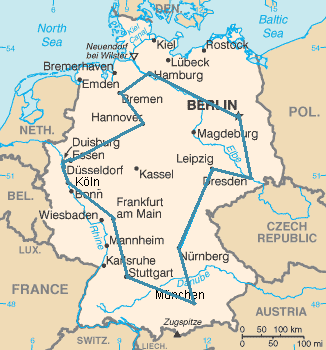
\includegraphics[width=0.9\textwidth]{1}
\column{0.5\textwidth}

This is the optimal traveling salesman route through the 15 largest cities in Germany. The indicated route is the shortest of all possible 43 589 145 600 options.
	\end{columns}
	\footnotetext{\url{https://commons.wikimedia.org/wiki/File:TSP_Deutschland_3.png}}
\end{frame}

\section{Hardness and complexity}
\begin{frame}
\frametitle{\insertsection}
\centering
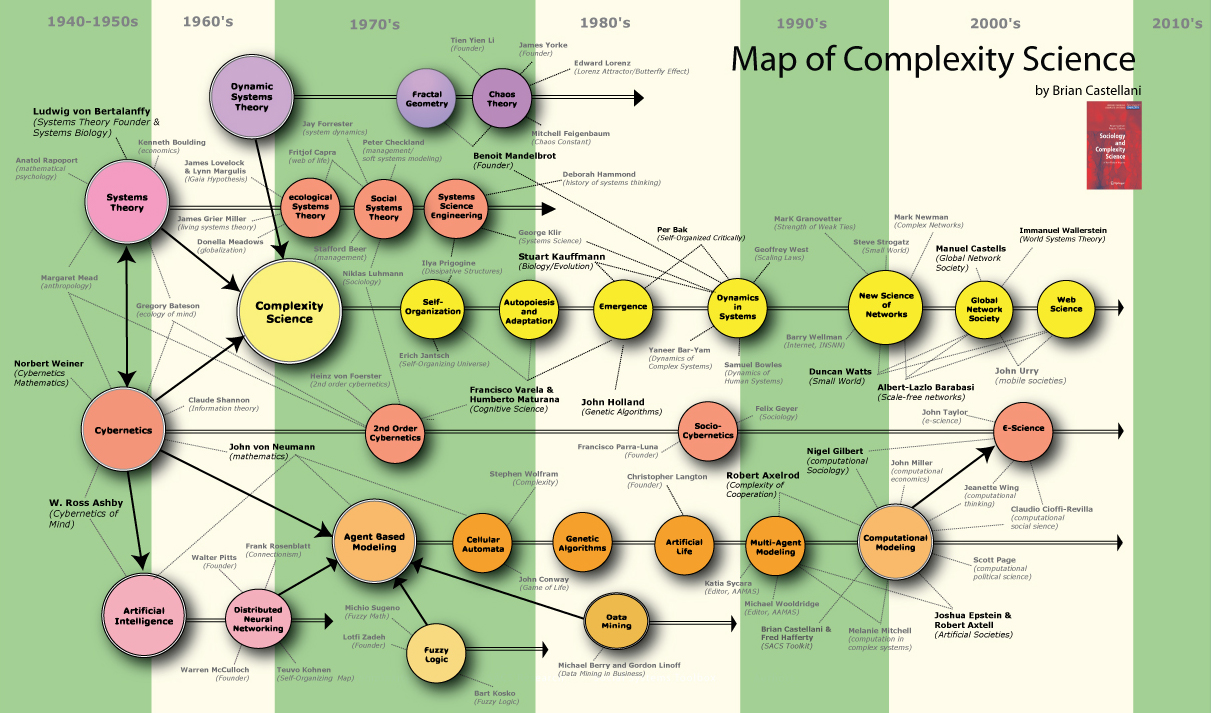
\includegraphics[width=0.8\textwidth]{2}\footnotetext{\url{https://serc.carleton.edu/NAGTWorkshops/complexsystems/definitions.html}}

Map of Complexity Science
\end{frame}

\section{The hardness of Math, English and fatherhood}
\begin{frame}
\frametitle{\insertsection}
\centering

\includegraphics[width=0.7\textwidth]{3}\footnotetext{\url{https://coolmompicks.com/blog/2017/06/10/funny-books-fatherhood-michael-ian-black-ben-falcone-jim-gaffigan/}}

	Fatherhood be like
\end{frame}

\section{Race, gender and brain chips}
\begin{frame}
\frametitle{\insertsection}
\centering

\includegraphics[width=0.8\textwidth]{4}\footnotetext{\url{https://www.express.co.uk/news/science/877457/brain-function-dementia-super-power-human-kernel}}

	Typical human with a brain chip
\end{frame}

\section*{Summary}
\begin{frame}
\frametitle{\insertsection}
\tableofcontents
\end{frame}

\begin{frame}{}
  \centering \Large
  \emph{Thank You for attention!}
\end{frame}
%\section{Описание модели}
%\begin{frame}
%\frametitle{\insertsection}
%
%Рассматриваемая модель представляет собой плоскую квадратную
%решётку, состоящую из $N$ узлов, в каждом из которых находится
%<<диполь>> с осью, перпендикулярной к плоскости решётки. Диполь
%может иметь две противоположные ориентации, так что общее
%число возможных конфигураций диполей равно $2^N$.
%
%С каждым узлом решётки (с целочисленными координатами $k,\,l$)
%свяжем переменную $\sigma_{kl}$, принимающую два значения
%$\pm 1$, соответствующие двум возможным ориентациям диполя.
%\end{frame}
%\section{Характеристики конфигурации решётки}
%\begin{frame}
%\frametitle{\insertsection}
%\begin{block}{Энергия}
%\[
%	E(\sigma)= -J \sum_{k,\,l=1}^{L} \left(\sigma_{kl}\sigma_{kl+1}
%	+\sigma_{kl}\sigma_{k+1l}\right)
%,\] 
%где $L$ --- число узлов в ребре решётки ($N=L^2$ ), а $J$ ---
%величина энергии взаимодействия пары соседних диполей.
%\end{block}
%\end{frame} 
%\begin{frame}
%\frametitle{\insertsection}
%\begin{block}{Статистическая сумма}
%\[
%	Z= \sum_{(\sigma)}^{} e^{-E(\sigma) /T}=\sum_{(\sigma)}^{} 
%	\exp \left[ \theta \sum_{k,\,l}^{} (\sigma_{kl}
%	\sigma_{kl+1}+\sigma_{kl}\sigma_{k+1l})\right] 
%,\] 
%где суммирование происходит по всем $2^{N}$ возможным конфигурациям, а также $\theta=J /T$.
%\end{block}
%\end{frame}
%\begin{frame}
%\frametitle{\insertsection}
%Т.\:к. $\sigma_{kl}^2=1$, то раскладывая экспоненту в ряд 
%по степеням $\theta$ получаем
%точное равенство
%\[
%	\exp(\theta \sigma_{kl}\sigma_{k'l'})=
%	\ch \theta + \sigma_{kl}\sigma_{k'l'} \sh\theta=
%	\ch \theta (1+ \sigma_{kl}\sigma_{k'l'} \th\theta)
%.\] 
%Поэтому
%\begin{multline*}
%	Z=\sum_{(\sigma)}^{} 
%	\exp \left[ \theta \sum_{k,\,l}^{} (\sigma_{kl}
%	\sigma_{kl+1}+\sigma_{kl}\sigma_{k+1l})\right] =\\=
%	(1-x^2)^{-N}\sum_{(\sigma)}^{} \prod_{k,\,l=1}^{L}
%	(1+x \sigma_{kl \sigma _{kl+1}})(1+x \sigma_{kl}\sigma_{
%	k+1l})
%,\end{multline*} 
%где $x=\th\theta$.
%\end{frame}
%\begin{frame}
%\frametitle{\insertsection}
%Итак,
%\[
%	Z=
%	(1-x^2)^{-N}\sum_{(\sigma)}^{} \prod_{k,\,l=1}^{L}
%	(1+x \sigma_{kl \sigma _{kl+1}})(1+x \sigma_{kl}\sigma_{
%	k+1l})
%.\] 
%
%Последнее выражение можно переписать в виде
%	\[
%		Z=(1-x^2)^{-N}S
%,\]
%где
%\[
%	S= \sum_{(\sigma)}^{} \prod_{k,\,l=1}^{L} (1+x \sigma_{kl}
%	\sigma_{kl+1})(1+x \sigma_{kl} \sigma_{k+1l})
%.\] 
%\end{frame}
%\section{Интерпретация суммы $S$}
%\begin{frame}
%\frametitle{\insertsection}
%Под знаком суммы
%\[
%	S= \sum_{(\sigma)}^{} \prod_{k,\,l=1}^{L} (1+x \sigma_{kl}
%	\sigma_{kl+1})(1+x \sigma_{kl} \sigma_{k+1l})
%\]
%имеем
%\[
%	\prod_{k,\,l=1}^{L} (1+x \sigma_{kl}
%	\sigma_{kl+1})(1+x \sigma_{kl} \sigma_{k+1l})
%\] 
%--- полином по переменным $x$ и $\sigma_{kl}$.
%\end{frame}
%\begin{frame}
%\frametitle{\insertsection}
%Имеем
%\[
%	\prod_{k,\,l=1}^{L} (1+x \sigma_{kl}
%	\sigma_{kl+1})(1+x \sigma_{kl} \sigma_{k+1l})
%.\]
%Заметим, что
%\begin{itemize}
%\item \only<1>{каждое $\sigma_{kl}$ может встретиться
%	в данном полиноме в степенях от нулевой до четвертой.}
%\only<2>{ после взятия суммы
%\[
%	S= \sum_{(\sigma)}^{} \prod_{k,\,l=1}^{L} (1+x \sigma_{kl}
%	\sigma_{kl+1})(1+x \sigma_{kl} \sigma_{k+1l})
%\]
%по всем $\sigma_{kl}=\pm 1$ члены, содержащие  нечётные степени
%$\sigma_{kl}$, обратятся в нуль, так что ненулевой вклад
%дадут только члены, содержащие $\sigma_{kl}$ в степенях
%0, 2, и 4.}
%\only<3>{ т.\:к. $\sigma_{kl}^0=\sigma_{kl}^2=\sigma_{kl}^4=1$,
%	то каждый член полинома, содержащий все переменные $\sigma_{kl}$ в чётных степенях, даст вклад в сумму $S$, пропорциональный
%числу конфигураций $2^N$ (после суммирования по всем
%конфигурациям $(\sigma)$).}
%\end{itemize}
%\end{frame}
%\begin{frame}
%\frametitle{\insertsection}
%Имеем
%\[
%	\prod_{k,\,l=1}^{L} (1+x \sigma_{kl}
%	\sigma_{kl+1})(1+x \sigma_{kl} \sigma_{k+1l})
%.\]
%Представим $x\sigma_{kl}\sigma_{kl+1}$ как вертикальное ребро,
%соединяющее <<диполи>> в узлах решётки $(k,\,l)$ и
%$(k,\,l+1)$, соответственно, а $x\sigma_{kl}\sigma_{k+1l}$,
%аналогично,
%как горизонтальное ребро.
%\begin{center}
%\incfig[0.7]{3}
%\end{center}
%
%\end{frame}
%\begin{frame}
%\frametitle{\insertsection}
%Имеем
%\[
%	\prod_{k,\,l=1}^{L} (1+x \sigma_{kl}
%	\sigma_{kl+1})(1+x \sigma_{kl} \sigma_{k+1l})
%.\]
%Каждому члену полинома можно однозначно поставить в соответствие
%совокупность рёбер, соединяющих некоторые пары соседних узлов
%решётки. Далее рассмотрим примеры таких соответствий.
%\end{frame}
%\begin{frame}
%\frametitle{\insertsection}
%\begin{center}
%\incfig[0.4]{4}
%\end{center}
%\[
%x^2 \sigma_{kl}\sigma_{k+1,l}^2 \sigma_{k+1,l-1}
%\] 
%\end{frame}
%\begin{frame}
%\frametitle{\insertsection}
%\begin{center}
%	\incfig[0.4]{5}
%\end{center}
%\[
%x^8 \sigma_{kl}^2\sigma_{k+1,l}^2 \sigma_{k+1,l-1}^2
%\sigma_{k,\,l-1}^4 \sigma_{k,\,l-2}^2\sigma_{k-1,\,l-1}^2
%\sigma_{k-1,\,l-2}^2
%\] 
%\end{frame}
%\begin{frame}
%\frametitle{\insertsection}
%\begin{center}
%	\incfig[0.4]{6}
%\end{center}
%\[
%x^{10} \sigma_{kl}^2\sigma_{k+1,l}^2 \sigma_{k+1,l-1}^2
%\sigma_{k,\,l-1}^2 \sigma_{k-2,\,l-1}^2\sigma_{k-1,\,l-2}^2
%\sigma_{k-1,\,l-3}^2\sigma_{k-2,\,l-3}^2\sigma_{k-2,\,l-2}^2
%\] 
%\end{frame}
%\begin{frame}
%\frametitle{\insertsection}
%Дадим геометрическую интерпретацию сделанным ранее замечаниям:
%\begin{itemize}
%\only<1>{\item $\sigma_{kl}^n\cdots,\ n=0,\,2,\,4\implies$ в каждом
%	узле графика заканчивается $0,\,2$ или 4 ребра (что
%	означает замкнутость графика, самопересечения
%допускаются)}
%\only<2>{\item каждый член полинома даёт вклад в сумму $2^N\implies$
%	сумму 
%\[
%	S= \sum_{(\sigma)}^{} \prod_{k,\,l=1}^{L} (1+x \sigma_{kl}
%	\sigma_{kl+1})(1+x \sigma_{kl} \sigma_{k+1l})
%\]
%	можно представить в виде
%	\[
%	S=2^N \sum_{r}^{} x^r g_r
%	,\] 
%где $g_r$ --- число замкнутых \alert{графиков}, составленных
%из (чётного) числа $r$ связей.}
%
%\end{itemize}
%\end{frame}
%\section{Ещё <<чуть-чуть>>}
%\begin{frame}
%\frametitle{\insertsection}
%Дальнейший расчёт состоит из двух этапов:
%\begin{enumerate}
%\item сумма по графикам указанного вида преобразуется в сумму
%	по всем возможным замкнутым петлям,
%\item получающаяся сумма вычисляется путём сведения к задаче
%	о <<случайных блужданиях>> точки по решётке.
%\end{enumerate}
%\end{frame}
%\section{Фазовый переход}
%\begin{frame}
%\frametitle{\insertsection}
%\only<1>{Окончательно, статистическая сумма будет иметь вид:
%\begin{multline*}
%	Z=2^N (1-x^2)^{-N}\times\\\times\prod_{p,\,q=0}^{L} \left[ 
%	(1+x^2)^2-2x(1-x^2)\left( \cos \frac{2\pi p}{L}+
%\cos \frac{2\pi q}{L}\right) \right] ^{1 /2} 
%.\end{multline*} }
%\only<1-2>{Термодинамический потенциал:
%\begin{multline*}
%	\Phi=-T \ln Z= - N T \ln 2 +N T \ln (1-x^2)-\\-
%	\frac{1}{2}T \sum_{p,\,q=0}^{L} \ln \left[ 
%	(1+x^2)^2-2x (1-x^2)\left( \cos \frac{2\pi p}{L}+
%\cos \frac{2\pi q}{L}\right) \right] 
%,\end{multline*} }
%\only<2-3>{или, переходя от суммирования к интегрированию
%\begin{multline*}
%	\Phi=-NT \ln 2+NT \ln(1-x^2)-\\- \frac{NT}{2(2\pi)^2}
%	\iint\limits_{0}^{2\pi}  \ln \left[ 
%	(1+x^2)^2-2x(1-x^2)(\cos \omega_1 +\cos \omega_2)\right] 
%	d\omega_1 d\omega_2
%.\end{multline*} }
%\only<3>{
%$\Phi$ имеет особую точку, когда аргумент логарифма нуль.
%Как функция от  $\omega_1$, $\omega_2$ этот аргумент минимален
%при $\cos \omega_1=\cos\omega_2=1$, когда он равен
%\[
%	(1+x^2)^2-4x(1-x^2)=(x^2+2x-1)^2
%.\]
%Это выражение имеет минимум, в котором оно обращается в нуль
%лишь при одном (положительном) значении $x=x_c=\sqrt{2} -1$;
%соответствующая температура $T_c \left( \th \frac{J}{T_c}=
%x_c\right) $ и является точкой фазового перехода.}
%\end{frame}
%\begin{frame}
%\frametitle{\insertsection}
%	Разложение $\Phi(t)$ по степеням $t=T-T_c$ 
%	вблизи точки перехода содержит наряду с регулярной
%	частью также и особый член. Заменяя регулярную
%	часть её значением при $t=0$, разлагая аргумент
%	логарифма вблизи его минимума по степеням
%	$\omega_1$, $\omega_2$ и $t$ и произведя интегрирование,
%	получим, что вблизи точки перехода термодинамический
%	потенциал имеет вид
%	\[
%		\Phi \approx a+ \frac{1}{2}b(T-T_c)^2
%		\ln |T-T_c|,
%	\]
%	где $a,\,b$ --- постоянные (причём $b>0$).
%	Сам потенциал непрерывен в точке перехода, а
%	теплоёмкость обращается в бесконечность
%	по закону
%	\[
%	C \approx -b T_c b \ln|T-T_c|
%	\] 
%	симметричному по обе стороны точки перехода.
%\end{frame}
%\section{Обсуждение результатов}
%\begin{frame}
%\frametitle{\insertsection}
%Из непрерывности первой производной термодинамического
%потенциала и скачка второй, заключаем, что в данной модели
%имеет место фазовый переход второго рода. На качественном
%уровне получается, что при температурах ниже критической
%большая часть диполей будет ориентирована одинаково,
%а при температурах выше --- диполей <<вверх>> и <<вниз>>
%будет поровну. Данная модель на качественном уровне
%описывает механизм ферромагнетизма (наличия намагниченности
%в отсутствии внешнего поля при достаточно низких температурах).
%\end{frame}
%\section{Приложения модели Изинга}
%\begin{frame}
%\frametitle{\insertsection}
%Введённая изначально для понимания природы ферромагнетизма, модель Изинга оказалась в центре разнообразных физических теорий, относящихся к критическим явлениям, жидкостям и растворам, спиновым стёклам, клеточным мембранам, моделированию иммунной системы, различным общественным явлениям и т. д. Кроме того, эта модель служит полигоном для проверки методов численного моделирования различных физических явлений.
%\end{frame}
%\section{Список литературы}
%\begin{frame}
%\frametitle{\insertsection}
%\begin{enumerate}
%	\item \emph{Паташинский А. З., Покровский В. Л.} Флуктуационная
%	теория фазовых переходов
%\item \emph{Ландау Л. Д., Лифшиц Е. М.} Статистическая физика
%\end{enumerate}
%\end{frame}
%\begin{frame}
%  \centering \Large
%  \emph{Спасибо за внимание!}
%\end{frame}
\end{document}
